\apendice{Especificación de diseño}

\section{Introducción}
En este apartado se describen los datos utilizados en el proyecto, como está formada la aplicación final y el diseño procedimental de la misma.

\section{Diseño de datos}
Este punto contiene de forma detallada los datos usados para entrenar con \emph{Detectron2}. También se habla de la aplicación y los ficheros que la forman.

\subsection{Radiografías Dentales}
Para poder entrenar el modelo de \emph{Detectron2} es necesario tener previamente imágenes con sus correspondientes JSON sobre las zonas que interesan al modelo que aprenda.

Es por ello, que el odontólogo Álvaro Zubizarreta Macho nos ha cedido un total de 10 radiografías junto con sus correspondientes JSON del diente y del nervio del que se desea conocer su longitud.

\subsection{Aplicación}
Las funciones de la aplicación se encuentran todas ellas en el fichero \texttt{funciones.py}. En su interior nos encontramos únicamente con una clase, la clase Predictor, la cual implementa un patrón \emph{Singleton} de modo que solo exista un objeto que apunto al modelo de la aplicación.

El resto del fichero son todo funciones encargadas de llevar a cabo las distintas operaciones necesarias en la aplicación.

\section{Diseño procedimental}
Este punto contiene el diagrama de secuencias que simula la iteración del usuario con la aplicación y los diferentes pasos que se dan, como se puede ver en la Figura \ref{secuencia}.

\begin{figure}[h]
 \centering
  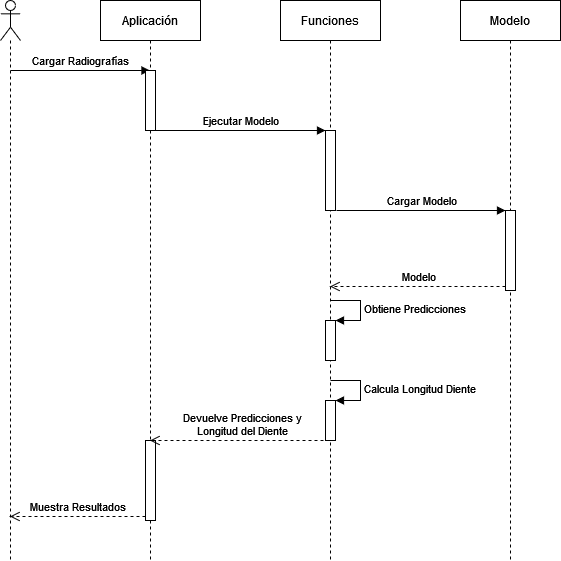
\includegraphics[width=0.8\textwidth]{img/DiagramaSecuencia.png}
 \caption{Diagrama de Secuencias de la Aplicación}
 \label{secuencia}
\end{figure}

\section{Diseño arquitectónico}
El diseño de la aplicación se podría dividir en tres partes principales: aplicación, funciones y modelo.

La aplicación es un \emph{notebook} encargado principalmente de cargar radiografías y mostrar los diferentes resultados de las mismas.

Las funciones, cuyo fichero tiene que estar en el mismo directorio que la aplicación, contiene todos los elementos necesarios para cargar el modelo, obtener las predicciones y calcular la longitud de los dientes. Gestiona todo el control de secuencia de código.

Por último, tenemos el modelo, que tiene que encontrarse en una carpeta con nombre \texttt{/output} dentro del directorio de la aplicación. Este modelo es el obtenido a lo largo proyecto con \emph{Detectron2}.
